%!TEX root = ../dissertation.tex
\begin{savequote}[75mm]
This is some random quote to start off the chapter.
\qauthor{Firstname lastname}
\end{savequote}

\chapter{Model and approach}

\todo{rivedere il titolo del capitolo}

SCALETTA:

* Visual branch
  * proposal 
  * object generator
* textual branch
  word embedding (w2v, glove)
* concept branch
* loss
* training and inference

\section{Model}

In the following sections we describe the model architecture, outlined
in Fig.\ref{fig:model-architecture}.

\begin{figure}
  \centering
  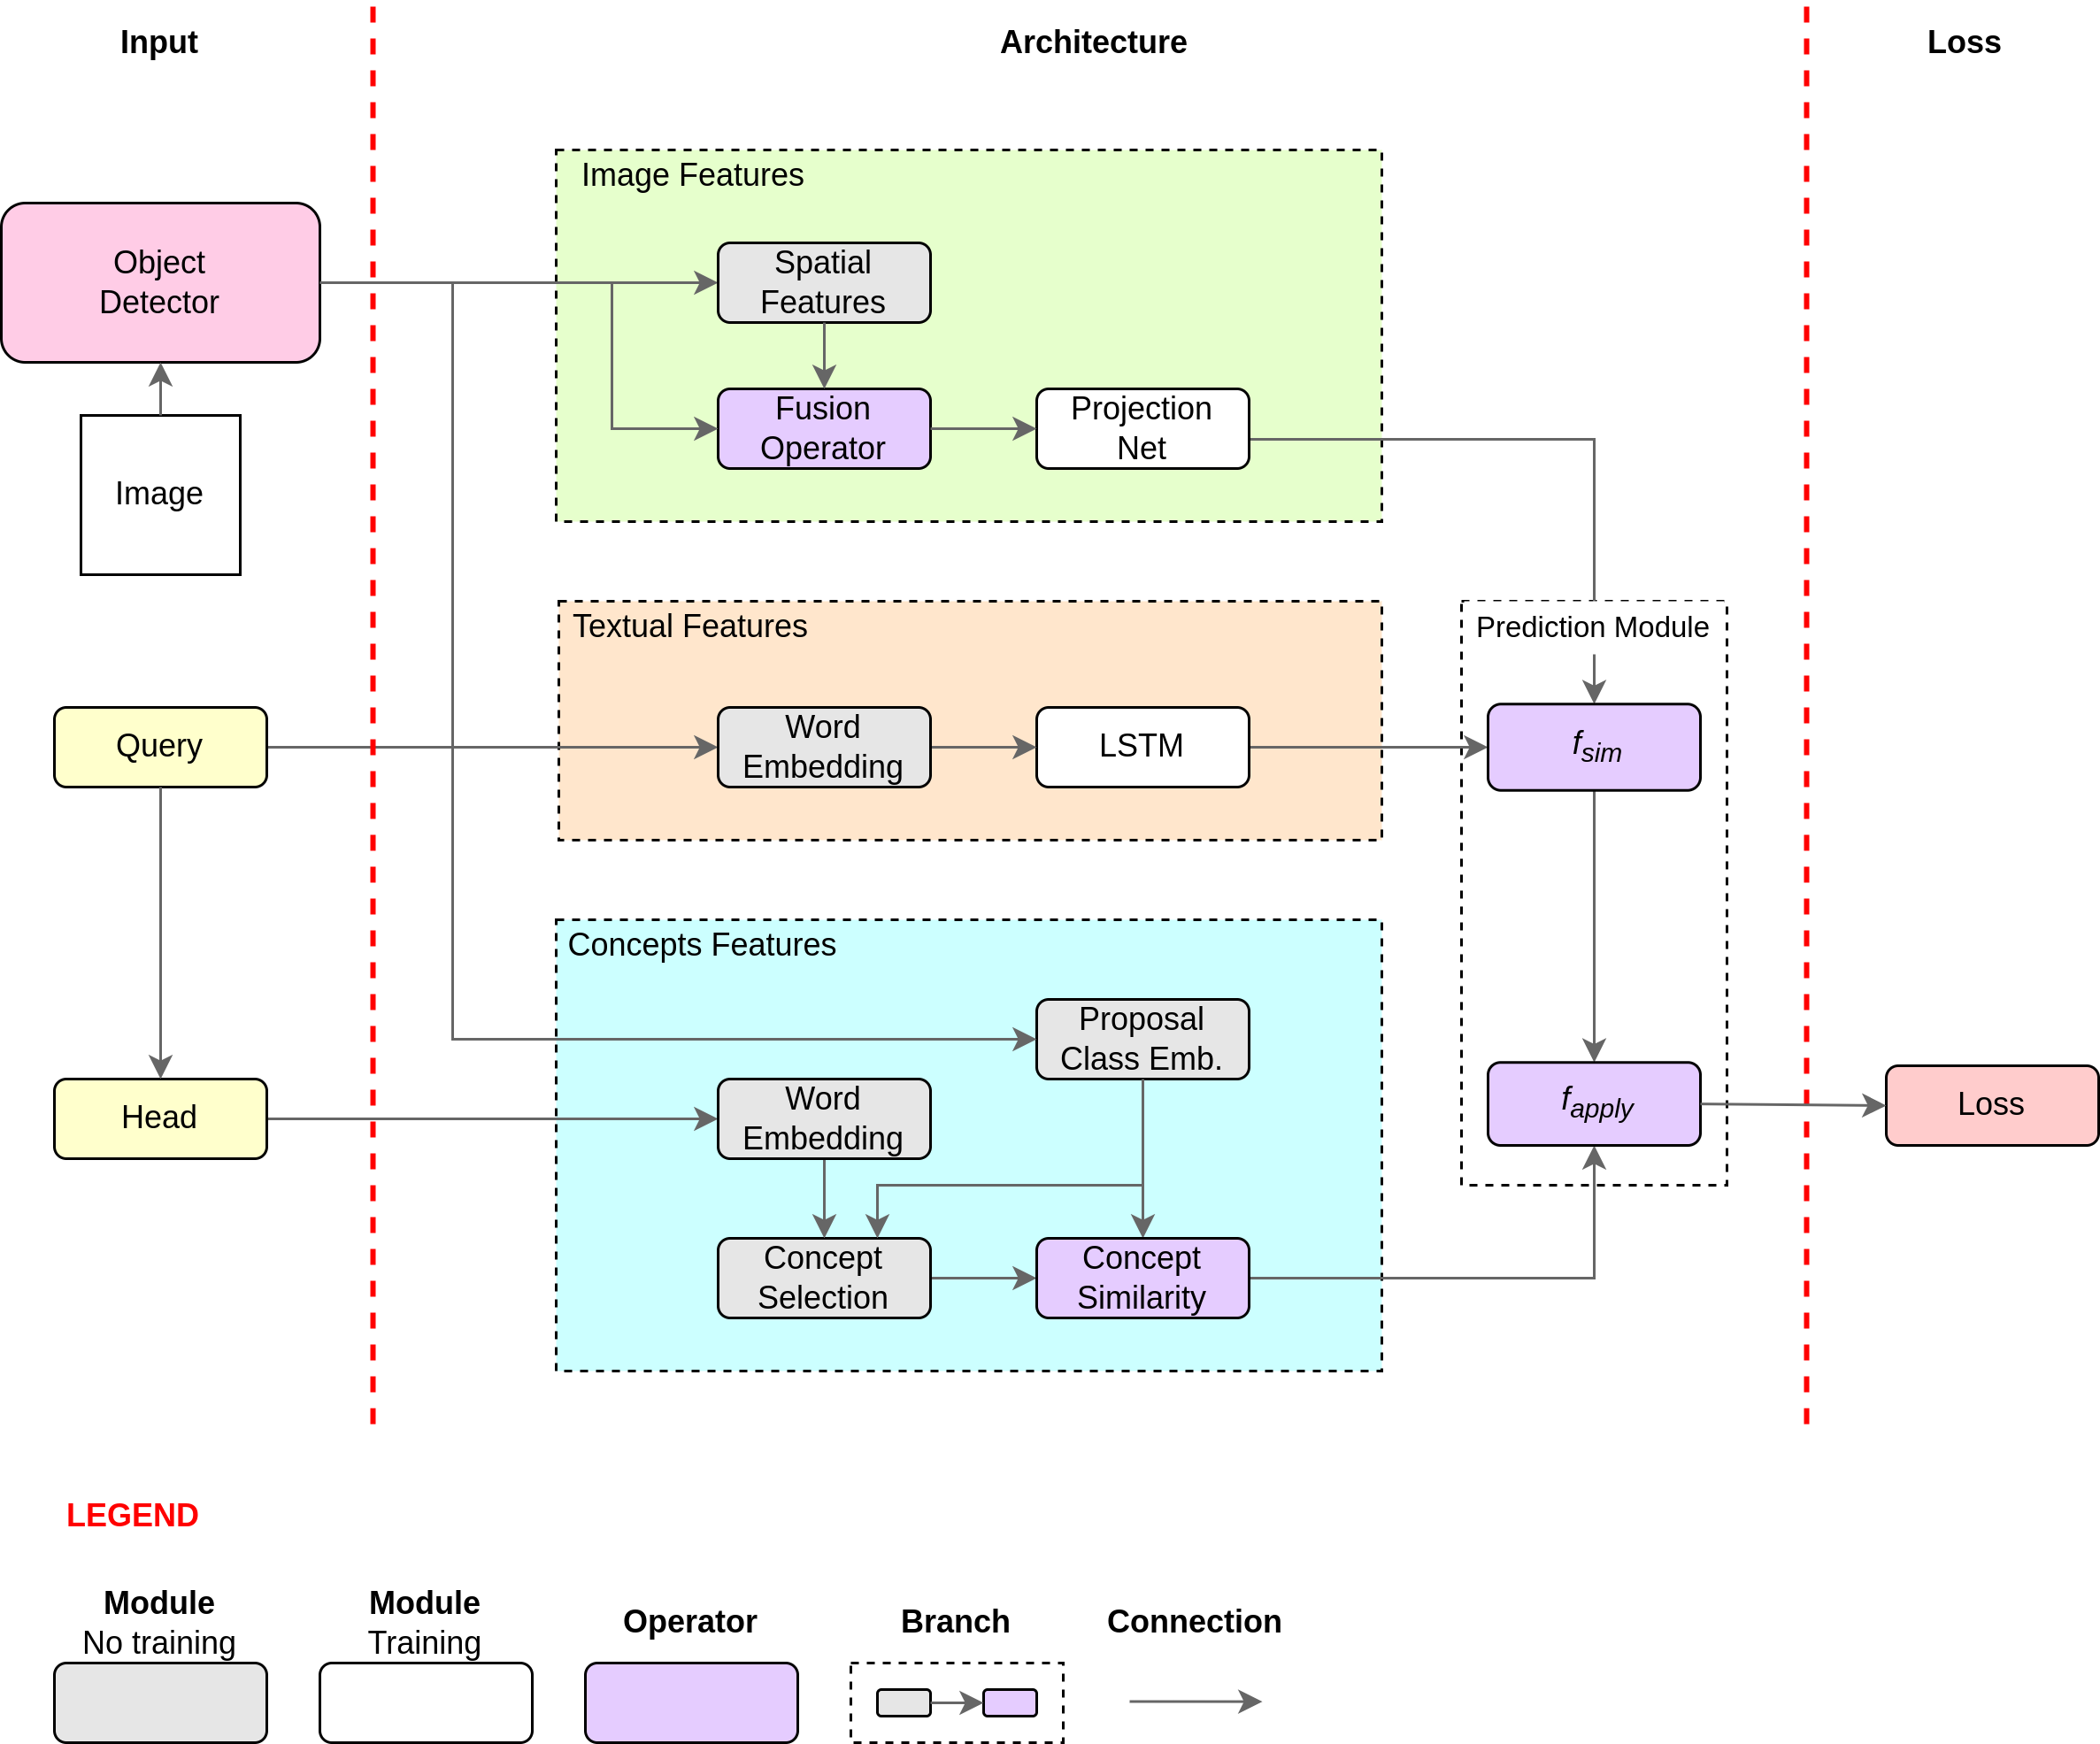
\includegraphics[width=1.0\textwidth]{figures/model-architecture.png}
  \caption[TODO]{Our model architecture overview. [WORK IN PROGRESS]}
  \label{fig:model-architecture}
\end{figure}

\subsection{Visual Branch}
\label{subsec:visual-branch}

Given an image $\bm{I}$, we extract a set of $k$ bounding box
proposals $\calP_{\bm{I}} = \{ \bm{p}_i \}^k_{i=1}$ by means of a
pre-trained object detector where $p_i \in \Rset^4$, jointly with
features $H^v = \{ \bm{h}^v_i \}^k_{i=1}$, where $\bm{h}^v_i \in
\Rset^v$. The features represent the internal object detector
activation values before the classification layers and regression
layer for bounding boxes. Moreover, our model extracts the spatial
features $H^s = \{ \bm{h}^s_i \}^k_{i=1}$, where $\bm{h}^s_i \in
\Rset^s$ from all the bounding boxes proposals, with the spatial
features for the proposal $\bm{p}_i$ defined as:
\begin{equation}
  \bm{h}^s_i = \left[ \frac{x1}{wt}, \frac{y1}{ht}, \frac{x2}{wt}, \frac{y2}{ht}, \frac{(x2 - x1) \times (y2 - y1)}{wt \times ht}  \right]
\end{equation}
where $(x1, y1)$ refers to the top-left bounding box corner, $(x2,
y2)$ refers to the bottom-right bounding box corner, $wt$ and $ht$ are
the width and height of the image, respectively. Both visual and
spatial features are then concatenated and projected, thus leading to
a set of new vectorial representations $H^{||} = \{ \bm{h}^{||}_{jz}
\}_{j \in [1, \ldots, m], z \in [1, \ldots, k]}$, where vectors
$\bm{h}^{||}_{jz}$ are defined as:
\begin{equation}
  \bm{h}^{||}_{jz} = \bm{W}^{||} \left( \bm{h}^s_z || L1(\bm{h}^v_z) \right) + \bm{b}^{||}
\end{equation}
where $||$ indicates the concatenation operator, $\bm{h}^{||}_{jz} \in
\Rset^c$, $\bm{W}^{||} \in \Rset^{c \times (s + v)}$ is a matrix of
weights, $\bm{b}^{||} \in \Rset^c$ is a bias vector, and $L1$ is the
L$1$ normalization function.

We also assume that the object detector returns, for each $\bm{p}_i$,
a probability distribution $Pr_{Cls}(\bm{p}_i)$ over a set $Cls$ of
predefined classes, i.e. the probability for each class $\zeta \in
Cls$ that the content of the bounding box $\bm{p}_i$ belongs to
$\zeta$. This information is typically returned by most of the object
detectors, and it will be used in Sec.~\ref{subsec:similarity-branch} to define the concept similarity.

\subsection{Textual Branch}

Regarding the textual features extraction, given a noun phrase
$\bm{q}_j$, initially all its words $W^{\bm{q}_j} = \{ w^{\bm{q}_j}_i
\}^l_{i=1}$ are embedded in a set of vectors $E^{\bm{q}_j} =
\{e^{\bm{q}_j}_i \}^l_{i=1}$ where $e^{\bm{q}_j}_i \in \Rset^w$, where
$w$ is the size of the embedding. Then, our model applies a LSTM
neural network (Sec.~\ref{subsec:gated-rnn}) to generate from the
sequence of word embeddings only one new embedding $\bm{h}^*_j$ for
each phrase $\bm{q}_j$. This textual features extraction is defined
as:
\begin{equation}
  \bm{h}^*_j = L1(LSTM(E^{\bm{q}_j}))
\end{equation}
where $\bm{h}^*_j \in \Rset^t$ is the LSTM output of the last word in
the noun phrase $\bm{q}_j$, and $L1$ is the L$1$ normalization
function.

\subsection{Similarity Branch}
\label{subsec:similarity-branch}

Along with visual and textual features we also compute a similarity
score between noun phrases and bounding boxes: the concept similarity
\cite{wang2019phrase}. The aim of such score is to capture the
semantic similarity between the content of a proposal and the concept
expressed by a phrase. But, instead of learning a complex multi-modal
mapping function between features, which is very difficult to realize
in weakly-supervised settings, we directly combine information given
by object detector and phrases. More precisely, we exploit those
information by leveraging on pretrained word embeddings. A good set of
word embeddings is able to capture, above all, the semantic similarity
between words, hence, words with same meaning should have similar
representation (Sec.~\ref{sec:word-embeddings}). Based on this
assumption, the similarity score can be trivially expressed as a
distance measure between two vectors in a space. Thus, the concept
similarity is none other than a distance measure applied to two word
embeddings. The first word embedding is extracted in a way that it can
express the content of a proposal. This information is made available
by the object detector, which usually return a probability
distribution over a set of classes, for each proposal
(Sec.~\ref{subsec:visual-branch}). We can easily gather the class that
best express proposal's content by simply taking the class associated
with the maximum prediction among the returned probability
distribution. This class is just a word (or, in some case a
combination of words), that can be naturally embedded in the word
embeddings space. The word embedding that express phrase concept,
instead, can be obtained by means of an NLP tool. Such tool we can
extract words that comply with some criteria, for example being a noun
or the head of the phrase. \todo{Apart from this, our model selects
the target words by considering the similarity with the bounding box
class label. - NON LO SPIEGHIAMO QUI MA SOTTO QUANDO ELENCO LE
STRATEGIE??}

Formally, we define $\EPI = \{\ePI_i \}^{k}_{i=1}$ the set of class
labels embeddings build on the set of proposal $\calP^{\bm{I}}$. Each
$\ePI_i$ is a feature vector representing the class label predicted
with maximum confidence by the object detector for the $i$-th
proposal. Then, given a noun phrase $\bm{q}_j$ along with
$E^{\bm{q}_j}$, we compute the concept similarity score for each
proposal $i$ and phrase $j$ as:
\begin{equation}
  \bm{S}^c_{ji} = \fsim \left( \xi_j, \ePI_i \right),
\end{equation}
where $\fsim$ is a similarity measure such us the cosine similarity,
and $\xi_j$ is the embedding representing the concept of the noun
phrase $\qj$. The new embedding $\xi_j$ can be computed with various
strategies that belongs to two different categories. In the first
group we can find operators that take into account the entire phrase
to generate a representative. A widely used strategy is to generate a
new embedding by averaging phrase's word embeddings:
\begin{equation}
  \xi_j = \frac{\sum^l_{i=1} \eqj_i}{| \Eqj |},
\end{equation}
however, there is an evidence that such averaging operations can
compromise the discriminativeness
\cite{wang2019phrase,datta2019align2ground}. If we consider instead a
single word as a representative for the phrase, a common strategy in
literature is to select the last word in the phrase
\cite{wang2019phrase}. Specially in English language, the last word of
a noun phrase is usually the head of the phrase. However, this
strategy relies on strong assumptions on language and how dataset is
built.\footnote{In \cite{wang2019phrase}, they show how the
\textit{last} strategy differs in performance on different dataset: on
Flickr30k Entities it is the second best strategy while in ReferIt it
doesn't even appear on the leaderboard.} More complex strategies,
instead, take into account external information, such us the
similarity wrt proposal class embeddings. Here, we compute the
similarity between word in noun phrase and proposal class embeddings
and then we select one word in the noun phrase with maximum similarity
wrt the detected concept in proposal:
\begin{equation}
  \xi_j = \argmax_{\eqj \in \Eqj} \{ \max g(\eqj) \},
\end{equation}
where
\begin{equation}
  g(\eqj) = \{ \fsim(\ePI, \eqj) \mid \ePI \in \EPI \}.
\end{equation}

\subsection{Prediction Module}

Finally, the model predicts the probability $\bm{P}_{jz}$ that a given
noun phrase $\qj$ is referrred to a proposal bounding box $\bm{p}_z$
as:
\begin{equation}
  \bm{P}_{jz} = \fsim ( \bm{h}^{||}_{jz} , \bm{h}^*_j ).
\end{equation}

As noted in \cite{chen2018knowledge}, concept similarity is a direct
consequence of the intrinsic knwoledge convoyed by the object
detector. Such score can be useful to down-weight unrelated proposals.
Its effectiveness is due to the fact that the word embedding usually
captures the semantic similarity between concept in phrase and the
content of the bounding box, and thus, let the model focuses on
relevant proposals. Thus, a straightforward improvement to our base
model would be to include this knowledge and exploit it for making
predictions. Hence, predictions can be enhanced by multiplying the
two, treating $\bm{S}^c_{jz}$ as a weight matrix:
\begin{equation}
  \bm{\hat{P}}_{jz} = \bm{S}^c_{jz} * \bm{P}_{jz}.
\end{equation}
At first glance, this approach seems very promising because we force
the model to return predictions ``on steroid'' when there is a
semantic relation between phrase and proposal or downweighted when
little similarity is found. However, this relies on the assumption
that the embedding space and similarity measure we are using for words
perfectly captures the semantic similarity between them, and this is
not true. Also, we assume that proposals are classified with no error
by the object detector, neither this is true. Under those hypotesis,
such application of concept similarity cannot be fruitful. 

An example my clarify our statement. We are given $\bm{S}^c \in
\Rset^{1 \times 2}$, $\bm{S}^c = [0.1, 0.2]$ for an example composed by a
phrase and two proposal, and we know that the bounding box to ground
with our prhrase is the first. The only way the model has to output
the first proposal as the best bounding box, i.e., the bounding box to
ground, is to predict a score $p_{0}$ which is at least the double of
$p_{1}$, because
\begin{equation}
  \bm{\hat{P}} = [0.1 * p_{0}, 0.2 * p_{1}]
\end{equation}
and hence
\begin{equation}
\begin{split}
0.1 * p_{0} > 0.2 * p_{1} & \iff p_{0} >  \frac{0.2}{0.1} * p_{1} \\
  & \iff p_{0} > 2 * p_{1}.
\end{split}
\end{equation}
Here, $p_{j} = \bm{P}_{0,j}$. Thus, with such scores $\bm{S}^c$, when
the model predicts $0.1$ for $p_1$, it must learn to predict $> 0.2$
for $p_0$, when it predicts $0.5$ for $p_1$, it must learn to predict
$1.0$ (the maximum) for $p_0$ and when it predicts a value $> 0.5$ for
$p_1$ there is no way to predict a greater score for $p_0$. In
conclusion, the model isn't really able to learn and its completely at
the mercy of similarity scores.

A more convenient way of applying concept similarity to prediction is
instead to compute the mean between two. Eventually, we can also put a
weight $\lambda \in [0 .. 1]$ in order to balance
contributions. Formally:
\begin{equation}
  \bm{\hat{P}}_{jz} = (1 - \lambda) * \bm{S}^c_{jz} + \lambda * \bm{P}_{jz}.
\end{equation}
The major benefit of this approach is that model predictions are not
constrained to values defined by concept similarity: they co-work to
the final predictions.

\section{Training}


In this section we present our loss function. For the sake of
presentation, we define in the following the loss terms referred to a
single example. The total loss is then obtained by summing up the
contributions of all examples in the training set.

Please note that in unsupervised settings, for a training example
$\left( \bm{I}, S \right)$ we are not given the query-proposal pair
set $\{ ( q^{gt}_j, p^{gt}_j ) \}^m_{j=1}$, where $m$ is the number of
noun phrases. To tackle this problem, in our work we adopt a very
simple strategy: we exploit concept similarity. Basically, we attract
representations whose concept similarity is above a certain treshold,
otherwise we want to repulse them. We define our oracle as:
\begin{equation}
  \bm{D}_{jz} =
  \begin{cases}
    1, & \bm{S}^c_{jz} > \alpha \\
    -1, & \text{otherwise}
  \end{cases},
\end{equation}
where $\bm{S}^c$ is the concept similarity matrix, $j$ is the
$\alpha$ is the threshold. This policy relies on the assumption that
concept similarity correctly captures the semantic relation between
query and proposal. $\bm{D}$ is the concept direction matrix.

Now, given a training example $\left( \bm{I}, S \right)$, where
$\cal{P}_{\bm{I}}$ the bounding box proposals set, we define the loss
function $\calL$ (for a single example) as:
\begin{equation}
  \calL = \frac{1}{m} \sum^m_{j=1} \Bigg( \frac{1}{k} \sum^k_{z=1} \floss ( \bm{P}_{jz}, \bm{D}_{jz} ) \Bigg)
\end{equation}
where $m$ in the number of noun phrases, $k$ is the number of proposal
bounding box, $\bm{P}_{jz}$ is the model predicted probability that
the noun phrase $\bm{q}_j \in \calQ$ refers to the image content
localized by $\bm{p}_z \in \calP_{\bm{I}}$. Our loss is scaled by $m$
and $k$ because number of noun phrase can change, but also number of
proposal. 

We optimize the model to learn features representation in the
similarity space, such that the depiction of $\bm{p}_z$ and $\bm{q}_j$
are neighbors when $\bm{D}_{jz}$ is $1$, perpendicular otherwise.
Formally:
\begin{equation}
  \floss^{\text{orthogonal}} \left( \bm{P}_{jz}, \bm{D}_{jz} \right) = - \bm{D}_{jz} \bm{P}^+_{jz} + \left( \bm{D}_{jz} \bm{P}^-_{jz} \right)^2,
\end{equation}
where $\bm{P}^+_{jz} = \One\left( \bm{D}_{jz} \right) \bm{P}_{jz}$
is the matrix that keeps predictions whose concept direction is over
the threshold and cancel the other, $\bm{P}^-_{jz} = \One\left( -
\bm{D}_{jz} \right) \bm{P}_{jz}$ instead cancels prediction with
concept similarity above threshold; $\One$ is the unit step function
\begin{equation}
  \One(x) =
  \begin{cases}
    1, & x \geq 0 \\
    0, & \text{otherwise}
  \end{cases}.
\end{equation}
<
Also in this case, some different strategies are available. Instead of
optimizing repulsed features to be perpendicular, one could also
exploit the similarity space and force them to be inversely
correlated. Another improvement would be to normalize the score by
number of bounding box with same class label. Indeed, due to the
long-tail distribution of bounding box class labels in dataset, some
representations are moved more than other: the normalization allows to
introduce a kind of equality.
